\documentclass[border=10pt]{standalone}

\usepackage{tikz}
\usepackage{tikzsymbols}
\usetikzlibrary{calc,patterns,shapes.geometric}

\def\centerarc[#1](#2)(#3:#4:#5){\draw[#1] ($(#2)+({#5*cos(#3)},{#5*sin(#3)})$) arc (#3:#4:#5);}

\begin{document}
	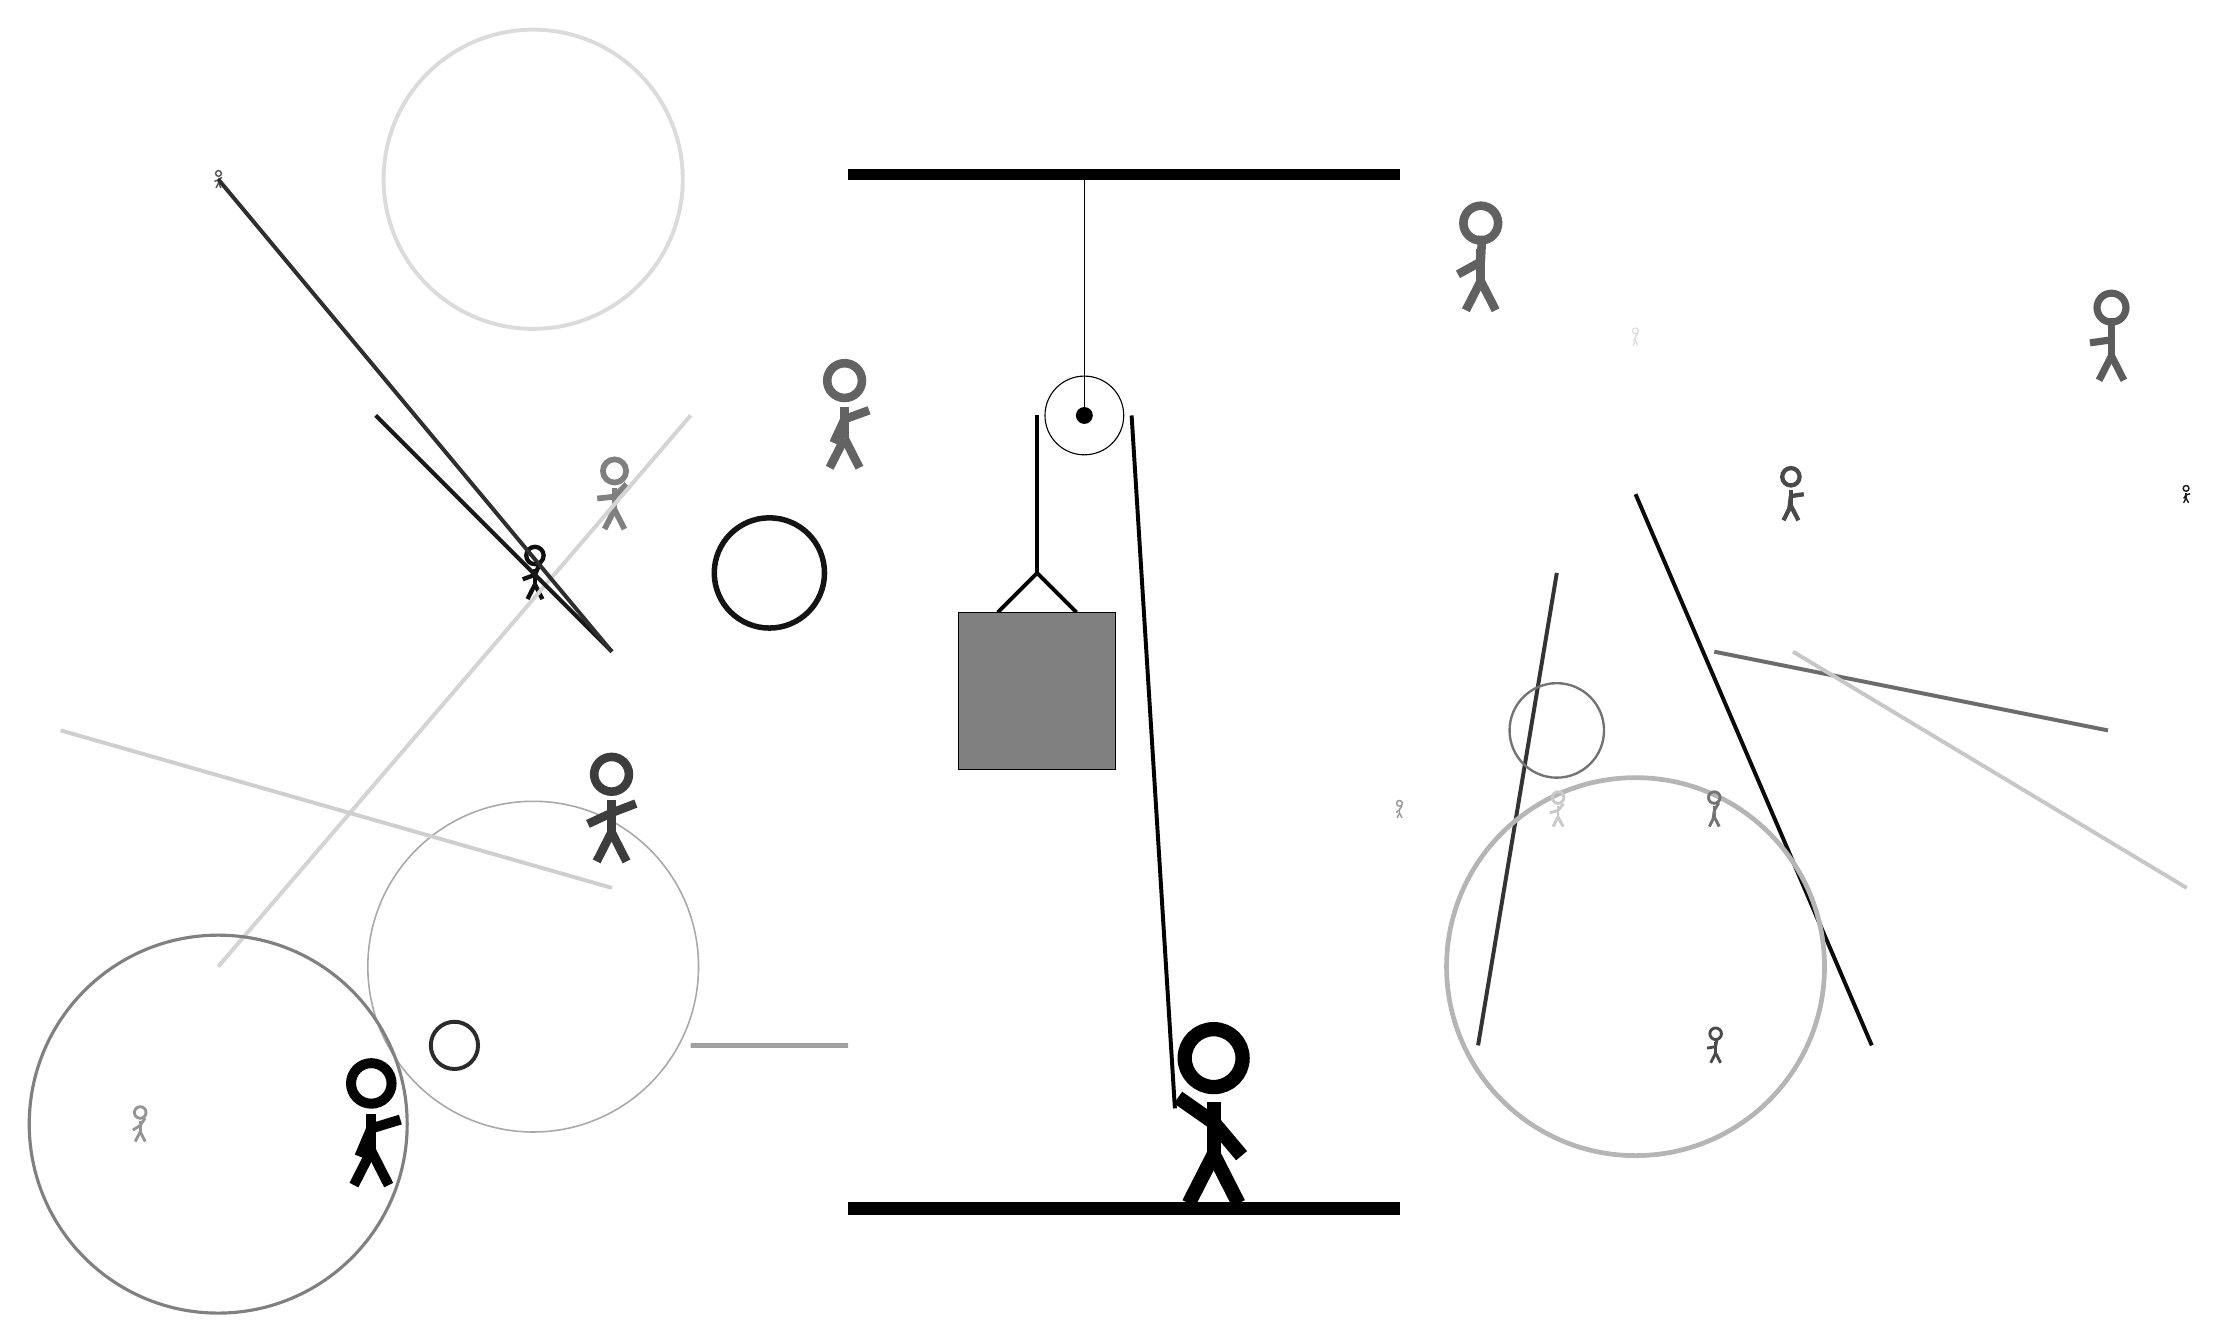
\begin{tikzpicture}
		%%%%% START %%%%%
		
		\draw[fill=black] (-2, 10) rectangle (5, 10.125);
		
		\draw (1, 7) circle (0.5);
		\draw[fill=black] (1, 7) circle (0.1);
		\draw (1, 10) -- (1, 7);
		
		\draw[line width=0.5mm] (-0.1, 4.5) -- (0.4, 5.0) -- (0.9, 4.5);
		\draw[fill=black!50] (-0.6, 4.5) rectangle (1.4, 2.5);
		
		\draw[line width=0.5mm] (0.4, 7) -- (0.4, 5.0);
		\centerarc[line width=0.5mm](1, 7)(0:180:0.6);
		\draw[line width=0.5mm](1.6, 7) -- (2.15, -1.8);
		
		\node at (2.6, -1.9) {\Strichmaxerl[10][-35][-50]};
		
		\draw[line width=0.5mm, color=black!58](9, 4) -- (14, 3);
		
		\node[line width=0.6mm, color=black!42] at (-11, -2) {\Strichmaxerl[2][33][56]};
		\draw[line width=0.5mm, color=black!96](8, 6) -- (11, -1);
		\node[line width=0.4mm, color=black!12] at (8, 8) {\Strichmaxerl[1][57][62]};
		\draw[line width=0.5mm, color=black!80](7, 5) -- (6, -1);
		
		\node[line width=0.5mm, color=black!62] at (6, 9) {\Strichmaxerl[6][29][87]};
		\node[line width=0.6mm, color=black!66] at (-10, 10) {\Strichmaxerl[1][20][35]};
		\node[line width=0.2mm, color=black!71] at (9, -1) {\Strichmaxerl[2][10][80]};
		\draw[line width=0.7mm, color=black!37] (-4, -1) rectangle (-2, -1);
		\node[line width=0.5mm, color=black!64] at (14, 8) {\Strichmaxerl[5][8][90]};
		\node[line width=0.3mm, color=black!89] at (15, 6) {\Strichmaxerl[1][56][15]};
		
		\node[line width=0.7mm, color=black!94] at (-6, 5) {\Strichmaxerl[3][20][67]};
		\node[line width=0.6mm, color=black!50] at (-5, 6) {\Strichmaxerl[4][6][46]};
		
		\node[line width=0.7mm, color=black!40] at (5, 2) {\Strichmaxerl[1][41][58]};
		\draw[line width=0.5mm, color=black!17](-4, 7) -- (-10, 0);
		\draw [line width=0.5mm, color=black!14](-6, 10) circle (1.9);
		\draw [line width=0.6mm, color=black!29](8, 0) circle (2.4);
		
		\node[line width=0.7mm, color=black!61] at (-2, 7) {\Strichmaxerl[6][65][20]};
		\draw [line width=0.2mm, color=black!34](-6, 0) circle (2.1);
		\draw [line width=0.3mm, color=black!55](7, 3) circle (0.6);
		\draw[line width=0.2mm, color=black!39] (-3, 7) rectangle (-3, 7);
		\draw[line width=0.5mm, color=black!90](-5, 4) -- (-8, 7);
		\node[line width=0.4mm, color=black!21] at (7, 2) {\Strichmaxerl[2][17][51]};
		\node[line width=0.6mm, color=black!99] at (-8, -2) {\Strichmaxerl[7][67][17]};
		\draw [line width=0.5mm, color=black!83](-7, -1) circle (0.3);
		
		\node[line width=0.4mm, color=black!55] at (9, 2) {\Strichmaxerl[2][82][59]};
		
		\draw [line width=0.7mm, color=black!92](-3, 5) circle (0.7);
		\draw[line width=0.5mm, color=black!82](-5, 4) -- (-10, 10);
		\draw[line width=0.5mm, color=black!19](-5, 1) -- (-12, 3);
		\node[line width=0.7mm, color=black!76] at (-5, 2) {\Strichmaxerl[6][25][21]};
		\node[line width=0.2mm, color=black!71] at (10, 6) {\Strichmaxerl[3][83][8]};
		\draw [line width=0.4mm, color=black!50](-10, -2) circle (2.4);
		\draw[line width=0.5mm, color=black!22](10, 4) -- (15, 1);
		
		
		\draw[fill=black] (-2, -3) rectangle (5, -3.15);
		
		%%%%% END %%%%%
	\end{tikzpicture}
\end{document}